\section{MOSFET Applications}
This part presents some applications using MOSFETs and most of them are EFETs. Students are proposed to implement the schematic and then, validate in PSPICE.
\subsection{MOSFET as a switch}
In this circuit arrangement an Enhancement-mode N-channel MOSFET is being used to switch a simple lamp “ON” and “OFF” (\textbf{could be replace by an resistor to simulate in PSPICE}).
\begin{figure}[!htp]
    \centering
    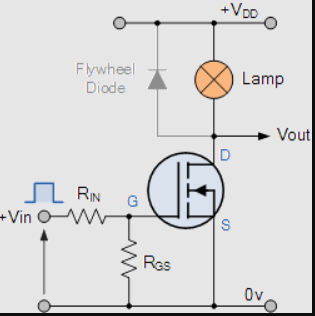
\includegraphics[width = 2.5in]{graphics/ex3/f1.png}
    \caption{EFET is used as a switch}
    \label{fet_app_1}
\end{figure}

The gate input voltage VGS is taken to an appropriate positive voltage level to turn the device and therefore the lamp load either “ON”, ( VGS = +ve ) or at a zero voltage level that turns the device “OFF”, ( VGS = 0V ).

If the resistive load of the lamp was to be replaced by an inductive load such as \textbf{a coil, solenoid or relay} a “flywheel diode” would be required in parallel with the load to protect the MOSFET from any self generated back-emf.

\textbf{Students are proposed to simulation this circuit with RIN = 4.7k and RGS = 47k and VIN is the TTL level (0V and 5V). The power supply for VDD can be set to 12V or 24V. Shortly explain the current passing through the load (a resistance 100Ohm replaced for the Lamp in the circuit)}.

Từ kết quả mô phỏng ta có: \( V_T = 0\, V, k = 10^{-5} \)

- Trường hợp \( V_{\text{in}} = 0 \):
\[
\frac{V_{\text{GS}}}{R_{\text{GS}}} = \frac{V_{\text{in}}}{R_{\text{GS}} + R_{\text{in}}} \quad \Rightarrow \quad I_\text{D} = k \cdot (V_\text{GS} - V_{\text{T}})^2 = 0 \, \text{A}
\]
\begin{figure}[!htp]
    \centering
    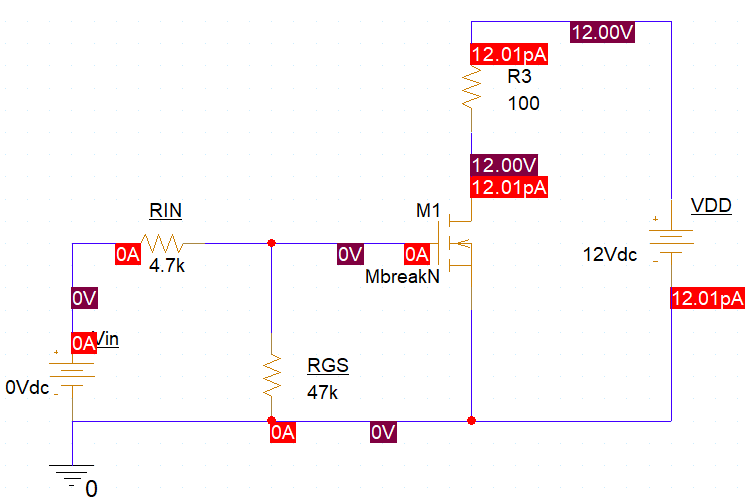
\includegraphics[width=0.7\textwidth]{graphics/ex3/f2.PNG}
\end{figure}

- Trường hợp \( V_{\text{in}} = 5 \, \text{V}\):
\[
V_\text{GS} =V_\text{in} \frac{R_\text{GS}}{R_{\text{GS}} + R_{\text{in}}} = 5 \cdot \frac{47k}{47k+4.7k} = \frac{50}{11}\, \text{V}
\]
\[
\Rightarrow I_D = k \cdot (V_\text{GS} - V_{\text{T}})^2 = 10^{-5}\cdot \left (\frac{50}{11} - 0 \right ) ^2 = 206.6 \, \mu\text{A}
\]
\begin{figure}[!htp]
    \centering
    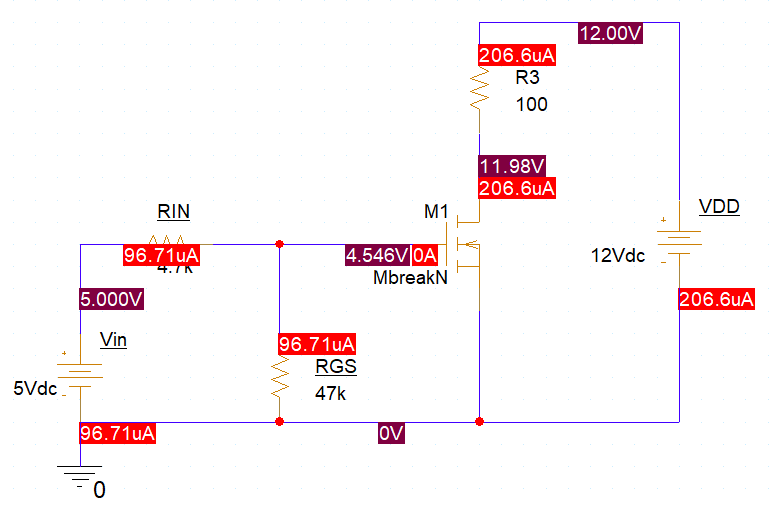
\includegraphics[width=0.7\textwidth]{graphics/ex3/f3.PNG}
\end{figure}






\subsection{MOSFET Motor Controller [Optional]}
\subsection{Complementary MOSFET Motor Controller [Optinal]}
